\documentclass[11pt,a4paper]{article}
\usepackage[margin=18mm]{geometry}
\usepackage{amsmath,amssymb,mathtools}
\usepackage{booktabs,array,enumitem}
\usepackage[dvipsnames]{xcolor}
\usepackage{graphicx,listings,tikz,float,needspace}
\usetikzlibrary{arrows.meta,positioning}
\usepackage[most]{tcolorbox}
\usepackage{hyperref}
\hypersetup{colorlinks=true,urlcolor=MidnightBlue,linkcolor=MidnightBlue}
\setlength{\parindent}{0pt}\setlength{\parskip}{4pt}
\newcommand{\course}{PHY4605 Computational Methods in Physics}
\newcommand{\units}[1]{\,\mathrm{#1}}
\newtcolorbox{keybox}{colback=RoyalBlue!5,colframe=RoyalBlue!65!black,boxrule=.7pt,arc=2mm}
\newtcolorbox{checkbox}{colback=ForestGreen!5,colframe=ForestGreen!55!black,boxrule=.7pt,arc=2mm}
\newtcolorbox{aibox}{colback=BurntOrange!7,colframe=BurntOrange!80!black,boxrule=.7pt,arc=2mm}
\lstdefinestyle{matlabstyle}{language=Matlab,basicstyle=\ttfamily\footnotesize,keywordstyle=\color{RoyalBlue!75!black},commentstyle=\color{ForestGreen!55!black},stringstyle=\color{BurntOrange!80!black},numbers=left,numberstyle=\scriptsize\color{black!50},numbersep=5pt,frame=single,rulecolor=\color{RoyalBlue!25},backgroundcolor=\color{RoyalBlue!3},showstringspaces=false,columns=fullflexible,keepspaces=true,breaklines=true}
\begin{document}
{\large\textsc{\course}}\\[-2pt]
{\small Learning Note \textbar\ Week 6}\par\vspace{4pt}
{\LARGE\bfseries Numerical Differentiation}\par\vspace{3pt}
\textit{Estimate a physical rate from nearby values, then check how well the numerical derivative matches a known reference.}

\begin{keybox}\textbf{Physical question.} A projectile follows a familiar vertical-position model. How can two nearby position values estimate its instantaneous vertical velocity at $t=1.0\units{s}$?\end{keybox}

\section*{Core learning outcomes}
\begin{enumerate}[nosep,leftmargin=5mm]
\item interpret a derivative as a physical rate and preserve its unit;
\item trace a forward-difference estimate for several supplied step sizes; and
\item validate a numerical derivative with an analytic reference and simple error.
\end{enumerate}

\section*{1. A derivative is a physical rate}
In physics, a derivative is not only a calculus symbol. It describes how one physical quantity changes when another changes. If vertical position $y$ is measured in metres and time $t$ in seconds, then
\[
\frac{dy}{dt}
\]
has unit metres per second. It is a vertical velocity.

The same idea appears elsewhere: $dT/dt$ is a heating or cooling rate, and $dV/dx$ is a spatial gradient of electric potential. Week 6 focuses on estimating such rates numerically when we have model values rather than directly using a symbolic derivative.

\begin{checkbox}\textbf{Prediction checkpoint.} At $t=1.0\units{s}$, a projectile launched upward at $20\units{m\,s^{-1}}$ should still be moving upward, but more slowly because gravity acts downward. Therefore $dy/dt$ should be positive and less than $20\units{m\,s^{-1}}$.\end{checkbox}

\section*{2. From a tangent slope to two nearby values}
The exact derivative is the local slope of the tangent. A forward difference replaces that tangent by a secant through two nearby points:
\[
\left.\frac{dy}{dt}\right|_{t=t_0}
\approx
\frac{y(t_0+h)-y(t_0)}{h}.
\]
Here $t_0$ is the target time and $h>0$ is the time separation between the two samples.

In words:
\begin{center}
\textbf{change in position} $\div$ \textbf{change in time} $\rightarrow$ \textbf{approximate velocity}.
\end{center}

The numerator has unit metres and the denominator has unit seconds, so the derivative estimate has unit m/s.

\begin{figure}[H]
\centering
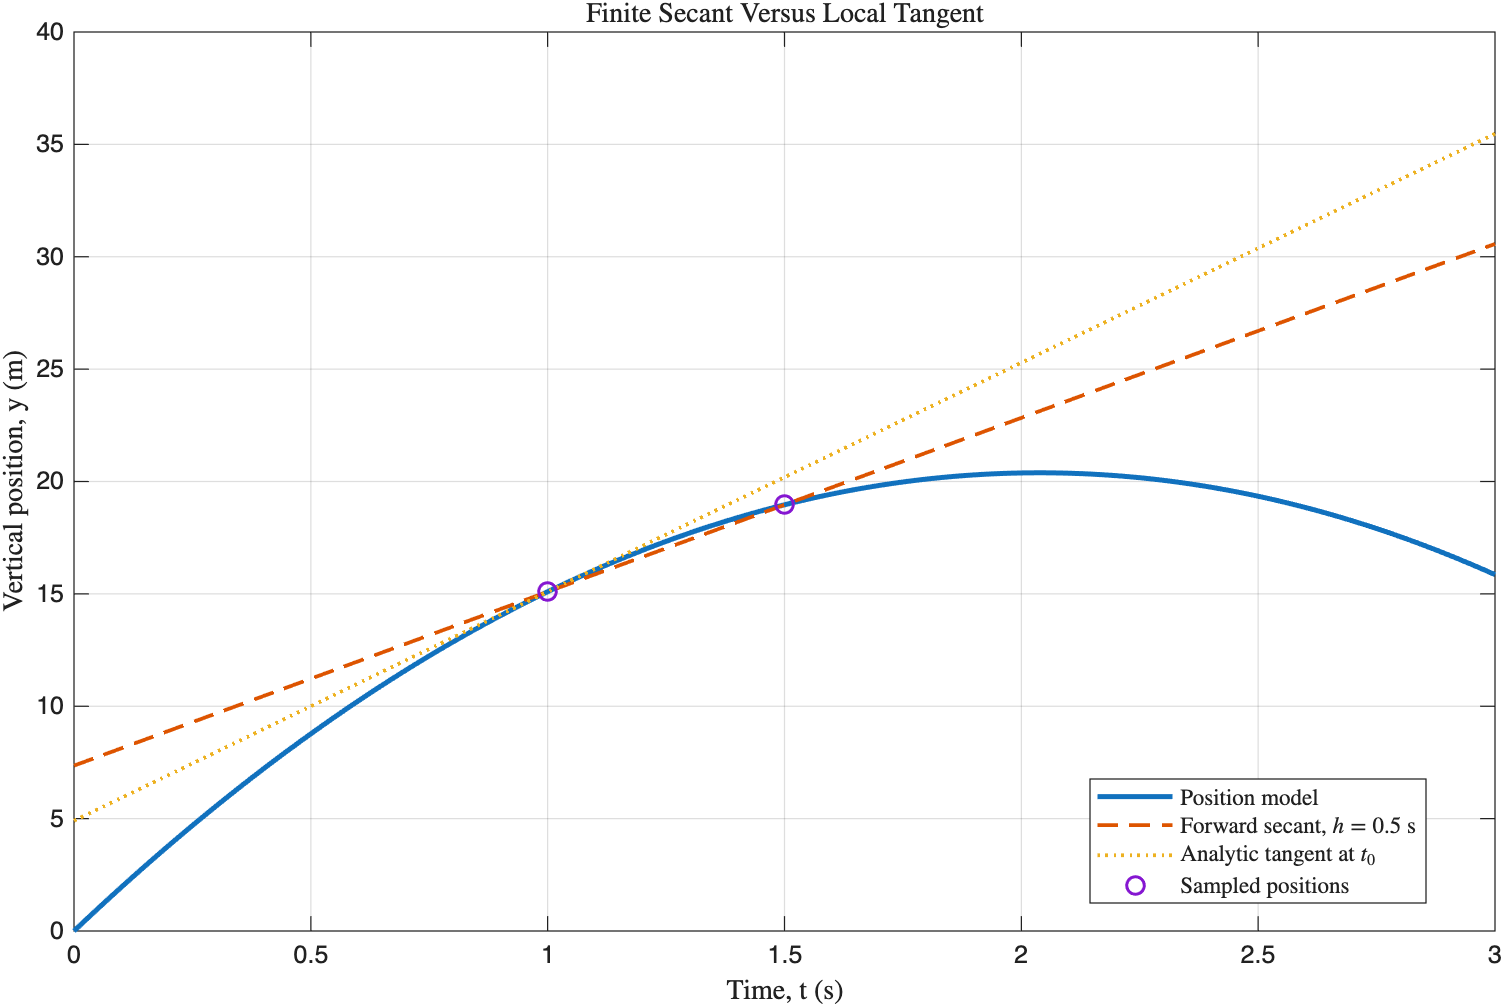
\includegraphics[width=.88\linewidth]{../matlab/assets/week06_forward_difference_geometry.png}
\caption{MATLAB-generated geometry for the Week 6 model. The forward-difference secant over a finite step approximates the local tangent slope at $t_0$.}
\end{figure}

\section*{3. Reuse a familiar vertical-motion model}
Use
\[
y(t)=y_0+v_0t-\frac{1}{2}gt^2,
\]
with
\[
y_0=0\units{m},\qquad v_0=20\units{m\,s^{-1}},\qquad g=9.81\units{m\,s^{-2}}.
\]
We want the derivative at
\[
t_0=1.0\units{s}.
\]
The analytic derivative is
\[
v(t)=\frac{dy}{dt}=v_0-gt,
\]
so the independent reference at the target time is
\[
v(1.0)=20-9.81(1.0)=10.19\units{m\,s^{-1}}.
\]
This analytic result is the validation reference, not the numerical method itself.

\section*{4. One forward difference by hand}
For $h=0.5\units{s}$,
\[
y(1.0)=15.095\units{m},\qquad y(1.5)=18.96375\units{m}.
\]
Therefore
\[
v_{\mathrm{FD}}(1.0)
=\frac{18.96375-15.095}{0.5}
=7.7375\units{m\,s^{-1}}.
\]
The sign and unit are physically sensible, but the estimate is lower than the analytic value $10.19\units{m\,s^{-1}}$. The finite interval from $1.0$ to $1.5\units{s}$ averages a changing velocity rather than sampling an exact tangent.

\section*{5. Pseudocode before MATLAB}
\begin{enumerate}[nosep,leftmargin=7mm]
\item choose the target time $t_0$ and one supplied positive step $h$;
\item evaluate the position model at $t_0$;
\item evaluate the same model at $t_0+h$;
\item subtract the two position values;
\item divide by $h$ to obtain the forward-difference estimate;
\item compare with the analytic derivative at the same $t_0$; and
\item repeat for the next supplied step size.
\end{enumerate}

\section*{6. Scaffolded MATLAB calculation}
\begin{lstlisting}[style=matlabstyle]
y0_m = 0;
v0_mps = 20;
g_mps2 = 9.81;
t0_s = 1.0;
h_s = [0.5 0.2 0.1 0.05];
y_now_m = y0_m + v0_mps*t0_s - 0.5*g_mps2*t0_s^2;
y_forward_m = y0_m + v0_mps*(t0_s+h_s) ...
    - 0.5*g_mps2*(t0_s+h_s).^2;
v_forward_mps = (y_forward_m-y_now_m)./h_s;
\end{lstlisting}
The important line is the final one: the change in position is divided element-by-element by the corresponding time step. The target time and physical model remain fixed while only $h$ changes.

\Needspace{18\baselineskip}
\section*{7. Compare a small set of step sizes}
The supplied Core step sizes give:

\begin{center}\small
\begin{tabular}{rrrr}
\toprule
$h$ (s) & $v_{\mathrm{FD}}$ (m/s) & absolute error (m/s) & relative error (\%)\\
\midrule
0.50 & 7.7375 & 2.4525 & 24.0677\\
0.20 & 9.2090 & 0.9810 & 9.6271\\
0.10 & 9.6995 & 0.4905 & 4.8135\\
0.05 & 9.94475 & 0.24525 & 2.4068\\
\bottomrule
\end{tabular}
\end{center}

For this smooth model and this supplied range, the estimate approaches the analytic value as $h$ becomes smaller.
The lecture Live Script also supplies an error-versus-step-size graph for Working exposure. Read that graph as evidence from one model and finite range, not as proof that arbitrarily tiny steps are always better.

\section*{8. Core validation: compare with the analytic derivative}
The required validation is a direct comparison at the same target time:
\[
v_{\mathrm{exact}}(1.0)=10.19\units{m\,s^{-1}}.
\]
For $h=0.05\units{s}$,
\[
v_{\mathrm{FD}}=9.94475\units{m\,s^{-1}},
\]
so the absolute error is
\[
|9.94475-10.19|=0.24525\units{m\,s^{-1}},
\]
and the relative error is approximately
\[
\frac{0.24525}{10.19}\times 100\%\approx 2.41\%.
\]

\begin{checkbox}\textbf{Validation statement.} The smallest supplied forward step gives a positive velocity with the correct unit and is within about $2.41\%$ of the known analytic velocity. This supports the numerical estimate for the stated model and target time.\end{checkbox}

\section*{9. Diagnose a runnable but wrong calculation}
A common defect is
\begin{lstlisting}[style=matlabstyle]
wrong_mps = (y_next_m - y_now_m)/t0_s;
\end{lstlisting}
The code runs, but the denominator is wrong. The two sampled positions are separated by $h$, not by $t_0$. Numerical correctness requires the denominator to represent the actual input interval between the two model values.

\begin{aibox}\textbf{Responsible-AI caution.} AI-generated differentiation code can be syntactically valid while using the wrong interval, mixing units, differentiating the wrong quantity, or comparing values at different target points. Check the two sample locations, denominator, derivative unit, and reference point before accepting the result.\end{aibox}

\section*{Working exposure: central difference}
A supplied central difference uses values on both sides of the target point:
\[
\left.\frac{dy}{dt}\right|_{t=t_0}
\approx
\frac{y(t_0+h)-y(t_0-h)}{2h}.
\]
For this quadratic position model, the central difference happens to reproduce the analytic derivative to floating-point precision. This special agreement should not be generalised to every physical model.

A supplied error-versus-step-size curve may also be inspected qualitatively. Extremely small steps are not guaranteed to improve every finite-precision calculation. Detailed truncation-error order and round-off analysis are Stretch topics, not Core Week 6 requirements.

\section*{Optional stretch}
Optional distinction-level extensions include deriving error order, analysing truncation and round-off in detail, or implementing higher-order difference formulas. Removing this section leaves the complete Core pathway intact.

\section*{Three takeaways}
\begin{enumerate}[nosep,leftmargin=6mm]
\item A numerical derivative estimates a physical rate from nearby values and must carry the correct derivative unit.
\item A forward difference uses a finite secant, so the choice of step size affects the approximation.
\item Validate the estimate against an analytic or supplied reference and report simple error before trusting it.
\end{enumerate}

\begin{keybox}\textbf{Preparation for the practical.} Be ready to transfer the same reasoning to vertical velocity, electric field from a potential gradient, and a cooling rate. For every context, identify the quantity being differentiated, the input variable, the derivative unit, the two sample locations, the step size, and the validation reference.\end{keybox}
\end{document}
